\everymath{\displaystyle}
%\documentclass[pdftex,a4paper]{article}
\documentclass[a4paper]{article}
%%classes: article, report, book, proc, amsproc

%%%%%%%%%%%%%%%%%%%%%%%%
%% Misc
% para acertar os acentos
\usepackage[brazilian]{babel} 
%\usepackage[portuguese]{babel} 
% \usepackage[english]{babel}
% \usepackage[T1]{fontenc}
% \usepackage[latin1]{inputenc}
\usepackage[utf8]{inputenc}
\usepackage{indentfirst}
\usepackage{fullpage}
% \usepackage{graphicx} %See PDF section
\usepackage{multicol}
\setlength{\columnseprule}{0.5pt}
\setlength{\columnsep}{20pt}
%%%%%%%%%%%%%%%%%%%%%%%%
%%%%%%%%%%%%%%%%%%%%%%%%
%% PDF support

\usepackage[pdftex]{color,graphicx}
% %% Hyper-refs
\usepackage[pdftex]{hyperref} % for printing
% \usepackage[pdftex,bookmarks,colorlinks]{hyperref} % for screen

%% \newif\ifPDF
%% \ifx\pdfoutput\undefined\PDFfalse
%% \else\ifnum\pdfoutput > 0\PDFtrue
%%      \else\PDFfalse
%%      \fi
%% \fi

%% \ifPDF
%%   \usepackage[T1]{fontenc}
%%   \usepackage{aeguill}
%%   \usepackage[pdftex]{graphicx,color}
%%   \usepackage[pdftex]{hyperref}
%% \else
%%   \usepackage[T1]{fontenc}
%%   \usepackage[dvips]{graphicx}
%%   \usepackage[dvips]{hyperref}
%% \fi

%%%%%%%%%%%%%%%%%%%%%%%%


%%%%%%%%%%%%%%%%%%%%%%%%
%% Math
\usepackage{amsmath,amsfonts,amssymb}
% para usar R de Real do jeito que o povo gosta
\usepackage{amsfonts} % \mathbb
% para usar as letras frescas como L de Espaco das Transf Lineares
% \usepackage{mathrsfs} % \mathscr

% Oferecer seno e tangente em pt, com os comandos usuais.
\providecommand{\sin}{} \renewcommand{\sin}{\hspace{2pt}\mathrm{sen}}
\providecommand{\tan}{} \renewcommand{\tan}{\hspace{2pt}\mathrm{tg}}

% dt of integrals = \ud t
\newcommand{\ud}{\mathrm{\ d}}
%%%%%%%%%%%%%%%%%%%%%%%%



\begin{document}

%%%%%%%%%%%%%%%%%%%%%%%%
%% Título e cabeçalho
%\noindent\parbox[c]{.15\textwidth}{\includegraphics[width=.15\textwidth]{logo}}\hfill
\parbox[c]{.825\textwidth}{\raggedright%
  \sffamily {\LARGE

Cálculo Numérico: Lista de Integração Numérica

\par\bigskip}
{Prof: Felipe Figueiredo\par}
{\url{http://sites.google.com/site/proffelipefigueiredo}\par}
}

Versão: \verb|20150526|

%%%%%%%%%%%%%%%%%%%%%%%%


%%%%%%%%%%%%%%%%%%%%%%%%
\section{Formulário}
Seja $I = \int_a^b f(x) \ud x$ a integral de $f(x)$ no intervalo
$[a,b]$. Seja $h=b-a$.

Pela regra do trapézio, podemos aproximar numericamente o valor de $I$
por:

\begin{displaymath}
  I \approx \frac{h}{2} \left( f(a) + f(b) \right)
\end{displaymath}

Pela regra dos trapézios repetidos, podemos aproximar numericamente o
valor de $I$ com:

\begin{displaymath}
  I \approx \frac{h}{2} ( f(x_0) + f(x_1) + f(x_1) + f(x_2) + \ldots
  f(x_{n-1}) + f(x_n) ) =
\end{displaymath}
\begin{displaymath}
  = \frac{h}{2} \left( f(x_0) + 2 f(x_1) + 2 f(x_2) +
    \ldots + 2 f(x_{n-1}) + f(x_n) \right)
\end{displaymath}

\section{Exercícios}

\begin{enumerate}
\item Encontre uma aproximação das seguintes integrais com o método
  dos trapézios repetidos, com a quantidade de subdivisões requerida:
  \begin{enumerate}
  \item $f(x)= x^2$, em $[1,2]$, com 4 subdivisões 
    % x=1:.25:2, f=x.^2, trapezios(f,[1 2],4)
  \item $f(x) = \sqrt{x}$ em $[1,2]$, com 5 subdivisões
    %x=1:.2:2, f=sqrt(x), trapezios(f,[1 2],5)
  \item $f(x) = \ln(x)$, em $[1,4]$, com 3 subdivisões
    % x=1:4, f=log(x), trapezios(f,[1 4],3)
  \item $f(x) = \sin x$, em $[-3.14,3.14]$, com 4 subdivisões
    % x=-3.14:1.57:3.14, f=sin(x), trapezios(f,[-3.14 3.14],4)
  \item $f(x) = 2^x$, em $[0,2]$, com 4 subdivisões
    % x=0:0.5:2, f=2.^x, trapezios(f,[0 2],4)
  \item $f(x) = \frac{1}{1+x}$, em $[0,1]$, com 2 subdivisões
    % x=0:0.5:1, f=1./(1+x), trapezios(f,[0 1],2)
  \end{enumerate}

\item Aproxime as seguintes integrais usando a regra dos trapézios,
  com um único trapézio, isto é, sem subdividir o intervalo de
  integração.
  \begin{enumerate}
  \item $\int_1^{1.5}x^2\ln x \ud x$
    % x=[1 1.5], f=x.^2 .*log(x), trapezios(f,[1 1.5],1)
  \item $\int_{1}^{1.6} \frac{2x}{x^2-4}\ud x$
    % x=[1 1.6], f=2.*x./(x.^2-4), trapezios(f,[1 1.6],1)
  \item $\int_{-0.25}^{0.25}\cos ^2 x \ud x$
    % x=[-0.25 0.25], f=cos(x).^2, trapezios(f,[-0.25 0.25],1)
  \end{enumerate}

\section{Problemas}
\item Considere a seguinte tabela:

  \begin{tabular}{c|ccccc}
    $x$ & 0.0 & 0.5 & 1.0 & 1.5 & 2.0\\
    \hline
    $f(x)$ & 0.000 & 1.770 & 0.207 & 0.005 & 0.143 \\ 
  \end{tabular}

  Use a regra dos trapézios repetidos para encontrar a integral para
  aproximar a integral $\int_0^2f(x) \ud x$.

%x=0:0.5:2, f=sin(x).^2.*cos(x).^2, trapezios(f,[0 2],4)

\item A função $f(x) = e^{(x^2)}$ não possui primitiva, que pode ser
  encontrada pelas técnicas de integração do Cálculo, mas sua integral
  definida pode ser aproximada numericamente. Encontre uma aproximação
  de $I=\int_0^1e^{x^2} \ud x$ usando a regra dos trapézios com 4
  subdivisões.

% x=0:0.25:1, f=exp(x.^2), trapezios(f,[0 1],4)

\item Como o logaritmo natural $\ln (x)$ é a primitiva de
  $\frac{1}{x}$, podemos aproximar o valor do logaritmo usando a
  integração numérica.
  \begin{enumerate}
  \item Encontre uma aproximação de $\ln (2)$ integrando numericamente
    $f(x)=\frac{1}{x}$ em $[1,2]$, usando um único trapézio (isto é:
    $h=1$).

    % x=[1 2], f= 1./x, trapezios(f,[1 2],1)

  \item Encontre a mesma integral numérica, usando 2 trapézios

    % x=1:0.5:2, f= 1./x, trapezios(f,[1 2],2)

  \item Use sua calculadora ou computador para encontrar o valor de
    $\ln (2)$ e calcule o erro absoluto entre as respostas dos itens
    anteriores e este valor.
  \end{enumerate}

\item (Burden \& Faires 2010 - adaptado) Uma chapa corrugada é
  construída comprimindo uma chapada de metal até que ela forme uma
  onda senoidal.

  \begin{center}
    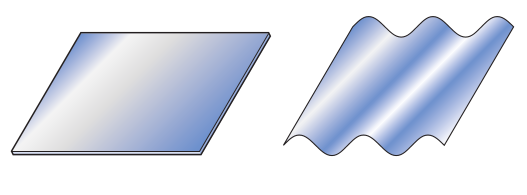
\includegraphics[width=0.4\textwidth]{corrugada}
  \end{center}

  Um cliente precisa que você construa uma chapa corrugada com meio
  metro de comprimento, e que a altura de cada onda seja de 1cm. O
  problema de encontrar o comprimento da chapa plana inicial é
  equivalente a determinar o comprimento da curva $f(x)=\sin x$. Do
  Cálculo Integral, sabe-se que este comprimento é dado pela integral
  $\int_0^{50}\sqrt{1-(f'(x))^2}\ud x = \int_0^{50}\sqrt{1-\cos^2 x}
  \ud x$. Qual é o comprimento da chapa plana necessário para produzir
  a chapa corrugada que o cliente deseja?

% x=0:10:50, f=sqrt(1-cos(x).^2), trapezios(f,[0 50],5)

\item (Burden \& Faires 2010 - adaptado) Um carro de corrida completa
  uma volta na pista em 84 segundos. Um radar portátil afere a
  velocidade do carro (em m/s) a cada 6 segundos, que estão
  representados na tabela a seguir.

  \begin{tabular}{c|ccccccccccccccc}
    tempo & 0 & 6 & 12 & 18 & 24 & 30 & 36 & 42 & 48 & 54 & 60 & 66 & 72 & 78 & 84\\
    \hline
    velocidade & 37 & 40& 45& 47& 44& 40& 36& 33& 30& 25& 23& 27& 31& 35& 37\\
  \end{tabular}

  Qual é o comprimento da pista?

% x=0:6:84
% f=[37 40 45 47 44 40 36 33 30 25 23 27 31 35 37 ]
% trapezios(f,[0 84],14)
% original (ft/s): f=[124 134 148 156 147 133 121 109 99 85 78 89 104 116 123]

\end{enumerate}


\end{document}
